\section{Parallel Architecture Design}
The program was designed to handle large graph as input (that implies large chromosome dimension). This was done by achieving data locality by modelling most of the application with \textit{Scanning} and \textit{Sorting} operation. As mentioned in \cite{algo-eng} RAM model fails to capture the running time for problems that have large data sets because of the I/O bottleneck. Indeed reading and writing data in sequential order or sorting the data to obtain requisite layout is less expansive than accessing data at random. This two operation, respectively \textit{std::for\_each} and \textit{std::sort}, were standardized and added to C++ until C++11 and are available inside the \textit{algorithm} header.

To exploit parallelism an initial analysis on the sequential version of the program was done. Each genetic operation was measured, by importing \textit{chrono} header library, to understand which part of the program needed to be parallelized and which not. This analysis was also useful to understand the proportion between the size of the graph and the time taken for each genetic algorithm operation. The following pie charts (figure \ref{fig:pie-chart-times}) were obtained by comparing each time spent by the operations that compose the algorithm, the number means the time taken in milliseconds to complete the operation. In both cases, the number of chromosomes taken into consideration was 2000 and the number of generation was 1.
\vspace{1.7em}

\begin{figure}[H]
	\centering
	\begin{minipage}[t]{0.55\linewidth}
		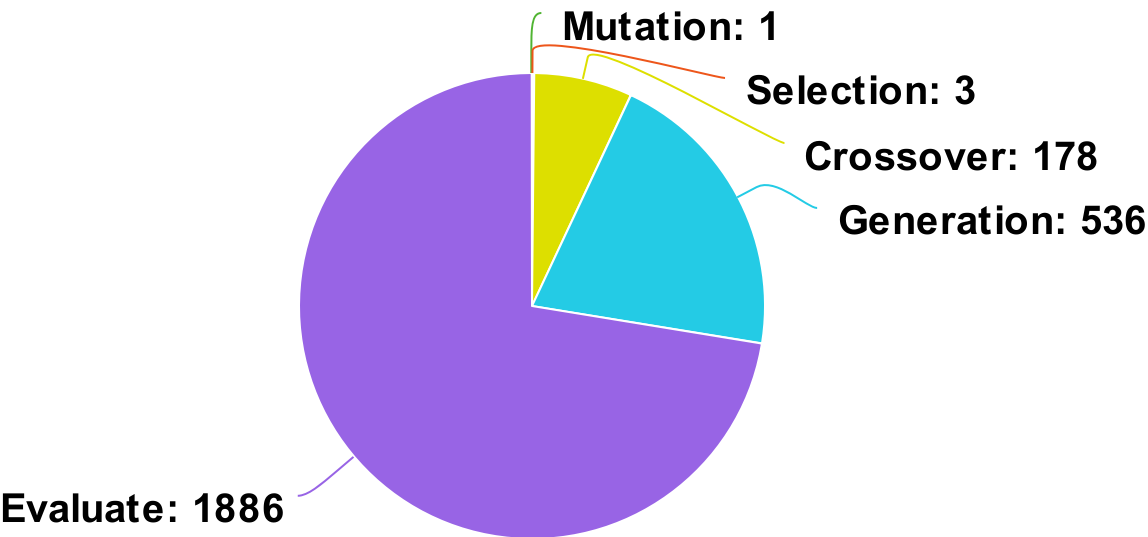
\includegraphics[width=\linewidth]{1000nodes6.png}
		\vspace{0.2em}
		\subcaption{1000 nodes} 
	\end{minipage}%
	\begin{minipage}[t]{0.57\linewidth}
		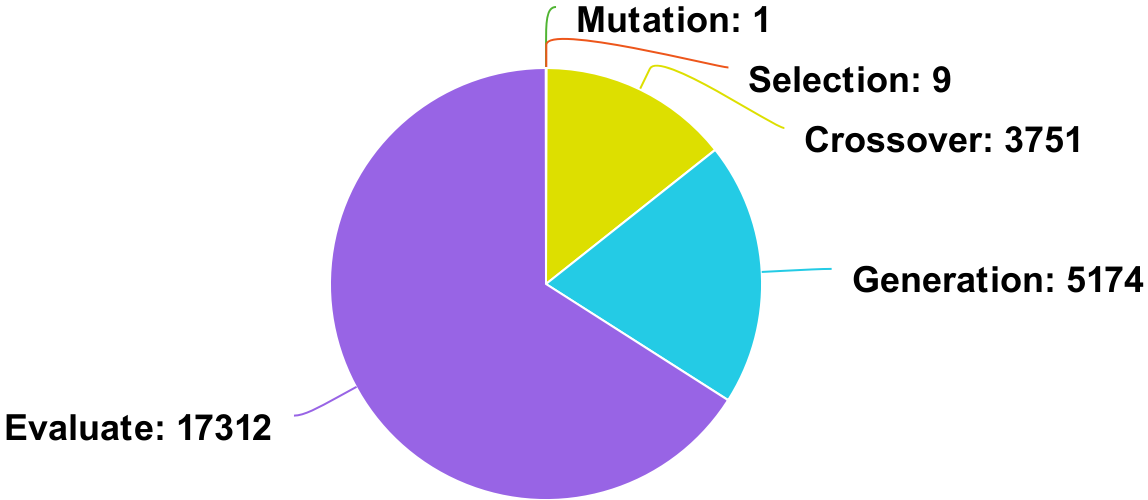
\includegraphics[width=\linewidth]{5000nodes5.png}
		\vspace{0.1em}
		\subcaption{5000 nodes}
	\end{minipage}
    \caption{}\label{fig:pie-chart-times}
\end{figure}

The first thing we noticed is that the most expansive operations are \textit{generation} (due to the random generation of the graph), \textit{evaluate} and \textit{crossover}.  Also, surprisingly, the selection phase that substitutes the old generation with the new one takes an insignificant amount of time. This is because all the index of the new population are sorted before the copy happens to exploit data locality and after the new generation is obtained (through \textit{Stochastic Universal Sampling} \cite{genetic-algorithm-tutorial}) the old generation is swapped with the new one, by moving the pointer, to avoid useless copy. 
\label{sez:architecture}

So, after the initial analysis I implemented the parallel versions by paying attention to the bottleneck created in \textit{evaluate}, \textit{generation} and \textit{crossover} phases. This was done by parallelizing the computation by splitting the works among multiple threads and then join the results obtained to proceed with the sequential computation of \textit{selection} and \textit{mutation} phases. Basically the high level structure of the program has the following operations form: 
\begin{figure}[H]
	\centering
	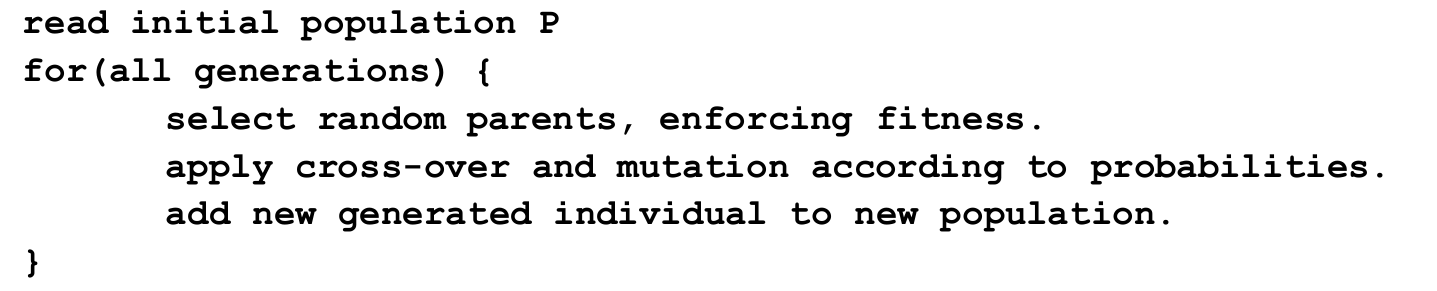
\includegraphics[width=0.75\textwidth]{geneticAlgorithmStructure.png}
	%\caption{Genetic algorithm structure}
\end{figure}
 
\subsection{Standard thread implementation}
Since exception safety is an essential aspect of C++ code, I decided to use a modern C++ approach to spawn the workers to compute the genetic algorithm heavy operations in parallel. Indeed, spawning threads with the standard constructor offer by \textit{std::thread} object doesn't guarantee exception safety and an exception launched by a single thread can terminate the whole application. Also the destruction of the threads, when an exception arises, is not guaranteed and the program can have leak memory thread problem (also known as dangling thread problem).

So, I decided to use \textit{std::async} to spawn the thread with \textit{std::launch::async} to launch it asynchronously, this action produce a result stored in a \textit{std::future<T>} and the operation to be done by each thread is passed in-place as a lambda function with all the parameters needed for the computation as input. This approach guarantee that even if an exception is raised by a thread and its \textit{std::future} object is destroyed the destructor will wait for the thread to complete, so the memory thread leak problem is avoided. 

The model used is the fork/join one, this was chosen because each chunk computed by a worker has the same size and amount of work (computational time speaking) to be done. So a dynamic load balancing of the work between threads was not needed. Indeed the communication arrow between masters node (heavy operation of the genetic algorithm) and the workers are implemented as ``chunks'' (in the code a \textit{std::pair<start,end>}) of the main data structure that has the current population saved in it. The implementation has the skeleton reported in figure \ref{fig:standardStructure}: 
\vspace{1.5em}
\begin{figure}[h]
	\centering
	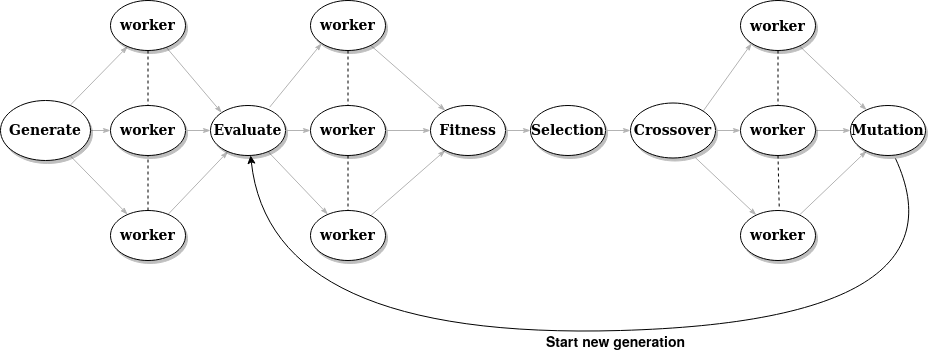
\includegraphics[width=1.1\textwidth]{standardMasterWorker.png}
	\vspace{0.15em}
	\caption{Standard C++ threads structure}
	\label{fig:standardStructure}
\end{figure}
\vspace{1em}

As we can see from figure \ref{fig:standardStructure} the first master worker spawning is done only at the beginning of the computation to speedup the random generation of the graph. This behaviour can be extended and modified, but basically the skeleton structure remains similar, to let the application parsing in parallel a file and create the graph. As mention above in \S \ref{sez:architecture} \textit{fitness} and \textit{selection} were designed as sequential computation because the time spent was too low (see \ref{fig:pie-chart-times} ) to obtain benefits exploiting parallelism.
 
\subsection{Fastflow implementation}
The version developed with Fastlow \cite{fastflow} was modelled using the information obtained from the analysis of the sequential algorithm (figure \ref{fig:pie-chart-times}). So, also in the Fastlow implementation the operations of \textit{generation}, \textit{evaluation} and \textit{crossover} were parallelized, moreover the communication between the emitters and collectors were chunks of indexes of chromosomes in the main data structure. The random generation of the graph was handled by creating a temporary farm with an emitter and a collector, but to save computational resources after the creation of the graph it is automatically deleted by the program. So the main skeleton of this version is composed by a pipeline composed by two farms (one for \textit{evalutation} and one for \textit{crossover}) and a sequential stage that computes the \textit{fitness} and \textit{selection} results. After creating the pipeline by injecting in the constructor the farms and the sequential node object the method \textit{wrap\_around()} is called to let the computation restarts from the initial emitter after all the current generation operations are done. 

\vspace{1.5em}
\begin{figure}[h]
	\centering
	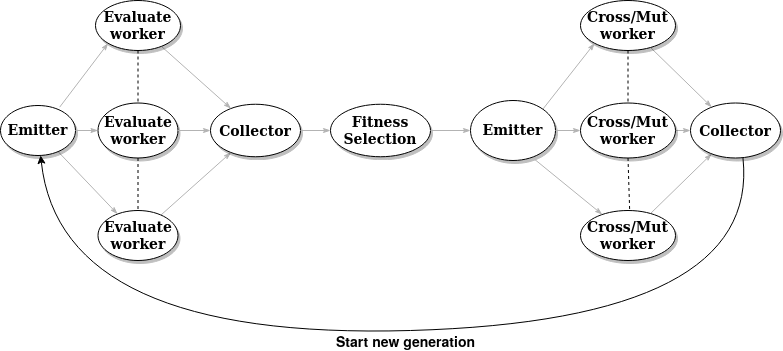
\includegraphics[width=1\textwidth]{fastflowMainStructure.png}
	\vspace{0.15em}
	\caption{Fastflow structure}
	\label{fig:fastflowStructure}
\end{figure}
\vspace{1em}

As we can see from figure \ref{fig:fastflowStructure} the sequential operations \textit{fitness} and \textit{selection} were merged in a single stage (node inside the pipeline) to save computational resources. Also every worker spawned by the second farm perform \textit{crossover} and immediately after that \textit{mutation} according to probabilities.

\section{Implementation details}
The project has three classes: \textit{fastflowTSP}, \textit{parallelTSP} and \textit{sequentialTSP}. If an object of \textit{Graph} type has been created and passed before in the constructor by calling the method \textit{Run} (and passing the parameters) the  algorithm starts. The user need to pass all the parameters by command line interface and then the program computes the three versions of the algorithm and for each of them the time spent is printed out. The only check is done on the number of workers by using \textit{std::thread::hardware\_concurrency()} method, if the user pass a number of workers that exceed the number returned by the method (so the supported thread of the machine are lower than the user specified threads), the number of thread is setted to the number returned by the method minus one. 